\scanpage{125}
\mspage{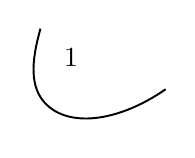
\begin{tikzpicture}[x=1cm,y=1cm,baseline=(n.base)]
\node (n) at (0.49,0.75) {\handwritten{1}};
\draw[line width=0.7pt] (0.10,1.12) .. controls (0.02,0.83) and (-0.05,0.49) .. (0.10,0.25) .. controls (0.36,-0.15) and (1.04,-0.10) .. (1.69,0.35);
\end{tikzpicture}}
% archive sheet number: 124

\handwritten{\unsure{Vallouin|Vallouir|Valloire|Vallouise} 18.\unsure{6|5|8}.1959}\\

Mon cher Serre;\\

Tate m'a écrit de son côté \deleted{pour} sur ses histoires de courbes elliptiques, et pour me demander si j'avais des idées sur une définition globale des variétés an\unsure{g|p|\deleted{a}g|\deleted{g}a}lytiques sur des corps valués complets. Je dois avouer que je n'ai pas du tout compris pourquoi ses résultats suggèreraient l'existence d'une telle définition, et suis encore sceptique. Je n'ai pas non plus l'impression d'avoir rien compris à son théorème, qui \deleted{\unsure{pour moi|pourquoi}} ne fait que exhiber par des formules brutales un certain isomorphisme de groupes analytiques; \deleted{et} on conçoit que d'autres formules tout aussi explicites en donneraient un autre pas plus mauvais (sauf preuve du contraire !)

J'ai réfléchi un petit peu à la partie 'infinitésimale' du groupe fondamental, juste assez pour me convaincre que ça existe et est raisonnable. Voici un contexte (certainement insuffisant d'ailleurs) où ça marche. On a un schéma $S$\inserted{\handwritten{connexe}} (par exemple un schéma algébrique sur un corps $k$), une catégorie auxiliaire $\underline{C}$ (par exemple la catégorie des schémas algébriques finis sur $k$), une catégorie \deleted{de} $\underline{G}$ dont les objets sont des $\underline{C}$-groupes, et les morphismes des morphismes de $\underline{C}$-groupes (par exemple les groupes algébriques finis sur $k$). On s\unsure{\deleted{a}u|\deleted{u}a}ppo\unsure{c|s}e que dans $\underline{C}$ les produits \deleted{\unsure{finis|fibrés}}\handwritten{fibrés} existent, et que $\underline{G}$ satisfait aux conditions suivantes: (i) $\underline{\mathbb{G}}$ est stable par produits, et si $u,v\unsure{;|:}G\handwritten{\longrightarrow}G'$ sont des morphismes dans $\underline{G}$, alors le noyau du couple $(u,v)$ i.e. le sous-groupe \deleted{\unsure{de|des}} maximum de $G$ où $u,v$ coïncidant -qui existe, car s'exprime par un produit fibré- est dans $\underline{G}$. (ii) Si $u:G\handwritten{\longrightarrow}G'$ est un morphisme dans $\underline{G}$, \deleted{alors il se décompo} le groupe image existe, est isomorphe à un quotient de $G$ comme il se doit, et est dans $\underline{G}$. (iii) Toute suite décroissante de sous-groupes \deleted{\unsure{d'un}} $\handwritten{\in}\underline{G}$ d'un $G\handwritten{\in}\underline{G}$ est stationnaire. On suppose donné de plus un foncteur covariant \deleted{$\unsure{F:\underline{G}|F:\underline{C}|F\longrightarrow\underline{G}}$} $F$ de $\underline{G}$ dans les \deleted{\unsure{G-groupes|S-groupes|k-groupes|K-groupes}} schémas en groupes sur $S$ (par exemple $G\handwritten{\longrightarrow}S\mathbin{\times}_{k}G$), et on suppose : (iv) Le foncteur $F$ commute aux produits, \inserted{\handwritten{aux}} noyaux de coupbes de morphismes, images (on pourra dire que $\unsure{F|\mathbb{F}}$ est ``exact''). (v) Si $H$ est \deleted{un} de la forme $F(G)$ $(G\handwritten{\in}\underline{G})$ alors $H$\inserted{\handwritten{est ``spécial'', i.e.}} admet une suite exacte
